%%%%%%%%%%%%%%%%%%%%%%%%%%%%%%%%%%%%%%%%%
%%% MG 1/4/2019 - logostic regression %%%
%%%%%%%%%%%%%%%%%%%%%%%%%%%%%%%%%%%%%%%%%

\clearpage

\section{Quick notes on logistic regression}\index{logistic regression}

Based in parts on these CMU \href{https://www.stat.cmu.edu/~cshalizi/uADA/12/lectures/ch12.pdf}{lectures}, \href{https://www.sagepub.com/sites/default/files/upm-binaries/21121_Chapter_15.pdf}{this} book chapter and wikipedia on \href{https://en.wikipedia.org/wiki/Logistic_regression}{logistic} and \href{https://en.wikipedia.org/wiki/Multinomial_logistic_regression}{multinomial logistic} regression.


\subsection{Logistic sigmoid}

In logistic regression the output variable $y \in \{0, 1\}$.
Still, we would like to use linear model in the form $\bw^T \bx$. 
However, the result of this linear model lives in $\mR$ while $y \in \{0, 1\}$.


We will therefore transform the $y$ variable.
First, instead treating it as discrete $\{0, 1\}$ we will treat it as continuous
in the interval $[0, 1]$ essentially indicating the probability $P(y=1) = \pi \in [0,1]$.
Another, and perhaps better, way of thinking about this is that the $y$ variable is generated from a Bernoulli distribution conditioned on $\bx$ with the expectation $\rE[y | \bx] = \pi$. What the model shall predict is not $y$ directly but rather $\rE[y | \bx] = \pi$.


Working with $\pi \in [0,1]$ is still not good enough since the outputs of the linear model are in $\mR$. We need to come up with an invertible transformation $g$ (\emph{link function}\index{link function}) so that $g(\rE(y | \bx)) = g(\pi) \in \mR$.

We start from odds\index{odds} of $y=1$ which is 
$$ \text{odds } = \frac{count(y=1)}{count(y=0)} = \frac{P(y=1)}{P(y=0)} = \frac{P(y=1)}{1- P(y=1)} = \frac{\pi}{1-\pi} \enspace .$$
The odds live in $[0, \infty)$.
To finally get to something which lives in $\mR$ we take the log of the odds $\log \text{odds} = \log \frac{\pi}{1-\pi} \in \mR$ also called \emph{logits}\index{logits}.
The linear model outputs therefore shall be the logits.
Good way to think about this is as the linear model for a transformation of the expected response. The output of the model is often indicated as $z$ and called the \emph{score}\index{score}. Here it is simply the linear model, but it could be preceded by a whole network with a final linear layer.
\begin{equation}
\log \frac{\pi}{1-\pi} = \bw^T \bx = z \enspace .
\end{equation}

It is rather easy to get the predictions in terms of the expectation of $y$, the probability $\rE(y | \bx) = \pi$, as the inverse of the logit \emph{link function}
\begin{eqnarray}\label{eq_logistic:sigmoid}
\frac{\pi}{1-\pi} & = & \exp(\bw^T \bx) \nn
\pi & = & \exp(\bw^T \bx) - \pi \exp(\bw^T \bx) \nn
\pi (1 + \exp(\bw^T \bx)) & = & \exp(\bw^T \bx) \nn
\rE(y | \bx) = \pi & = & \frac{\exp(\bw^T \bx)}{1 + \exp(\bw^T \bx)} = \frac{1}{1 + \exp(- \bw^T \bx)} = \sigma(\bw^T \bx) \enspace ,
\end{eqnarray}
where $\sigma : \mR \to [0,1]$ is the \emph{logistic sigmoid}\index{logistic sigmoid}\index{sigmoid} function.

\begin{figure}[h]
\centering
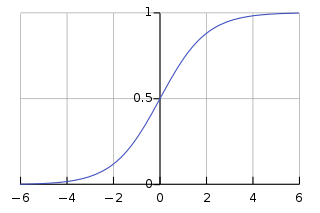
\includegraphics[width=5cm]{logistic_sigmoid.png}
\caption{Logistic sigmoid; source Wikipedia}
\end{figure}

\subsection{Cross-entropy loss}

For the binary $y$ the conditional probability distribution $p(y|\mathbf{x})$ is Bernouli with the conditional expectation $\pi = \rE(y | \mathbf{x})$. We can formulate the logistic regression problem objective as maximizing the likelihood of $\bw$ over the training set 
\begin{equation}
\max_{\bw} \prod_i^n \pi_i^{y_i} (1-\pi_i)^{1-y_i} \enspace ,
\end{equation}
where $\pi_i = \sigma(\bx_i^T \bw)$ from equation \eqref
{eq_logistic:sigmoid}.

We can instead minimize the negative log likelihood also called the \textbf{cross-entropy loss}\index{cross-entropy loss}
\begin{equation}
\min_{\bw} \sum_i^n - y_i \log \pi_i - (1-y_i) \log (1-\pi_i) \enspace ,
\end{equation}

Recall the definition of cross-entropy\index{cross-entropy}
\begin{equation}
H_p(q) = -\sum_c^C p(y_c) \log q(y_c) \enspace ,
\end{equation}
where $y$ is a random variable with C categories and $p$ and $q$ are two different distributions.

\subsection{Multi-class classification}

When we have more than 2 classes, we consider a linear model of the form $\bx^T \bw_c = z_c$ with specific parameters $\bw_c$ for each class and $z_c$ the per-class \emph{scores}\index{score}.

We can arrive at multinomial logistic regression following similar logic as in the binary case where we decompose the multiple categories $c = 1, \ldots, C$ into a set of $C-1$ dummy variables with the last category as the default pivot.

For each class we have the odds against the pivot as
\begin{equation}
\text{odds}_c = \frac{count(y=c)}{count(y = C)} = \frac{P(y=c)}{P(y =C )} = \frac{\pi_c}{\pi_C} \enspace .    
\end{equation}

The scores $z_c$ are the log-odds, the logits
\begin{equation}
z_c = \log \frac{\pi_c}{\pi_C} = \bx^T \bw_c
\end{equation}
from which we get
\begin{equation}
\pi_c = \pi_C \, \exp(\bx^T \bw_c) \qquad \text{for all } c=1, \ldots, C-1
\end{equation}


Because probabilities some to one, we have 
\begin{equation}
\pi_C = 1 - \sum_c^{C-1} \pi_c = 1 - \sum_c^{C-1} \pi_C \, \exp(\bx^T \bw_c) = 1 -  \pi_C \sum_c^{C-1} \exp(\bx^T \bw_c)
\end{equation}
and therefore 
\begin{equation}\label{eq_logistic:multinomial}
\pi_C = \frac{1}{1+\sum_c^{C-1} \exp(\bx^T \bw_c)} \qquad \pi_c = \frac{\exp(\bx^T \bw_c)}{1+\sum_c^{C-1} \exp(\bx^T \bw_c)}
\end{equation}

This is obviously equal to the binary logistic sigmoid in case of just two classes where $\pi_c =  P(y=1)$ and $\pi_C = P(y=0)$.

\paragraph{Soft-max} To get the \emph{soft-max}\index{soft-max} function instead of fixing one category as a pivot we treat all the probabilities evenly. This will in the end lead to overparametrization because we do not treat one class as the default.

As above, we have for the probabilities of each class
\begin{equation}
\pi_c = \frac{1}{Z} \, \exp(\bx^T \bw_c) \qquad \text{for all } c=1, \ldots, C \enspace ,
\end{equation}
which is now valid for all classes and where $Z$ is a common normalizing constant.

Since probability has to sum to $1$ we have
\begin{eqnarray}
1 = \sum_c^C \pi_c & = &  \frac{1}{Z} \sum_c^C \exp(\bx^T \bw_c) \nn
Z & = &   \sum_c^C \exp(\bx^T \bw_c) \nn
\pi_c & = & \frac{\exp(\bx^T \bw_c)}{\sum_c^C \exp(\bx^T \bw_c)} \enspace .
\end{eqnarray}

The coefficients in the soft-max are redundant (not uniquely identifiable), because the values of the soft-max will not change if we add a constant vector $\alpha$ to each of the parameters vector
\begin{equation}
\frac{\exp(\bx^T (\bw_c + \alpha))}{\sum_c^C \exp(\bx^T (\bw_c + \alpha))} = 
\frac{\exp(\bx^T \bw_c) \exp(\bx^T \alpha)}{\exp(\bx^T \alpha) \sum_c^C \exp(\bx^T \bw_c)} = \frac{\exp(\bx^T \bw_c)}{\sum_c^C \exp(\bx^T \bw_c)} \enspace . 
\end{equation}
If we fix $\alpha = -\bw_C$ to the parameters of the last class we get
\begin{equation}
\pi_C = \frac{\exp(\bx^T (\bw_C -\bw_C))}{\sum_c^C \exp(\bx^T (\bw_c -\bw_C))} = \frac{1}{1 + \sum_c^{C-1} \exp(\bx^T (\bw_c -\bw_C))} 
\end{equation}
and 
\begin{equation}
\pi_c = \frac{\exp(\bx^T (\bw_c -\bw_C))}{\sum_c^C \exp(\bx^T (\bw_c -\bw_C))} = \frac{\exp(\bx^T (\bw_c -\bw_C))}{1 + \sum_c^{C-1} \exp(\bx^T (\bw_c -\bw_C))} \enspace ,
\end{equation}
which is the same result as in equation \eqref{eq_logistic:multinomial} with the shifted weight vectors.


% https://en.wikipedia.org/wiki/Multinomial_logistic_regression

% https://chrisyeh96.github.io/2018/06/11/logistic-regression.html


% softmax overparametrized

